\section*{H3}
Sei M TM wie folgt:\\
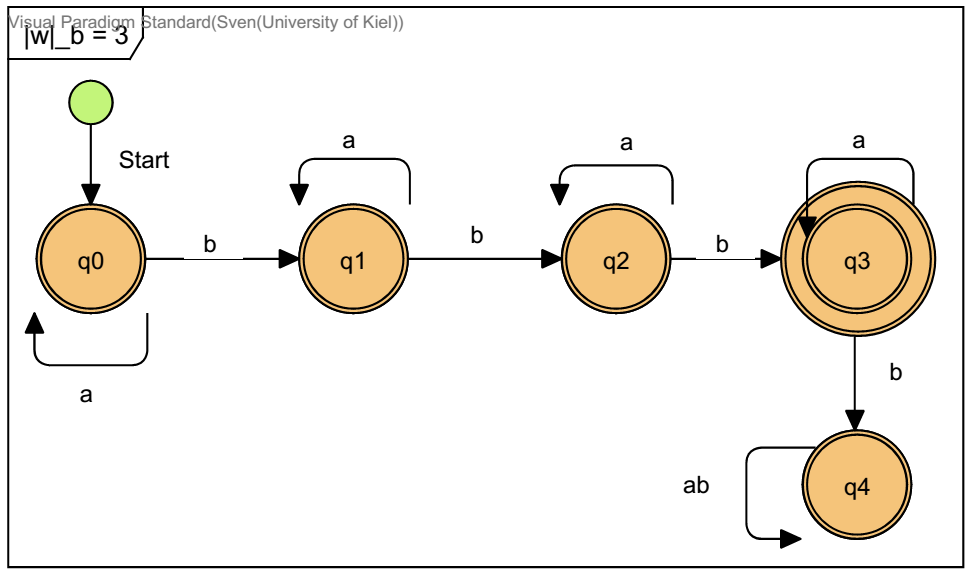
\includegraphics[scale=0.8]{part/TGIS08A03}
Beweis dass  $L(M)=L$:\\
Seien $u,v,x,y$ $\in a^* $ und $t \in \Sigma^*$\\
$\hat{\delta}(q_0,ubv)= \hat{\delta}(\delta (\hat{ \delta} (q_0,v),b), u) = \hat{\delta}(\delta (q_0,b), u) = \hat{\delta}(q_1, u) = q_1$ was nicht akzeptierend ist und $|ubv|_b=1$ $ubv\notin L$\\
\\
$\hat{\delta}(q_0,ubvbx)=\hat{\delta} ( \delta( \hat{\delta}(\delta (\hat{ \delta} (q_0,u),b), v),b),x) =\hat{\delta} ( \delta( \hat{\delta}(\delta (q_0,b), v),b),x) =\hat{\delta} ( \delta( \hat{\delta}(q_1, v),b),x) = \hat{\delta} ( \delta( q_1,b),x) = \hat{\delta} ( q_2),x) = q_2 $ was nicht akzeptierend ist und $|ubvbx|_b=2$ $ubvbx\notin L$\\
\\
$\hat{\delta}(q_0,ubvbxby)=\hat{\delta} ( \delta(\hat{ \delta} (q_0,ubvbx),b),y) = \hat{\delta}(\delta ( q_2),b),y) =\hat{\delta}(q_3,y)= q_3 $ was akzeptierend ist und $|ubvbxby|_b=3$ $ubvbxby\in L$\\
\\
$\hat{\delta}(q_0,ubvbxbybt)=\hat{\delta}(\delta ( \hat{\delta}(q_0,ubvbxby),b),t)=\hat{\delta}(\delta (q_3,b),t)=\hat{\delta}(q_4,t) = q_4  $ was nicht akzeptierend ist und $|ubvbxbybt|_b>3$ $ubvbxbybt\notin L$\\
\\
Somit sind alle $|w|_b$ Fälle abgedeckt und nur $|w|_b=3$ wird von M akzeptiert somit gilt $L(M)=L$


